\chapter{Theory}\label{chap:cms}


One of the most compelling questions in participle physics today is the hierarchy problem. The Randall Sundrum Kaluza Klein model proposes a solution in which the Planck scale is located on one membrane and the TeV scale a distance L away in a fourth spatial dimension. 

\begin{figure}[h]
	\centering
	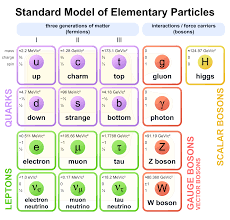
\includegraphics[width=0.5\textwidth]{figures/sm_blocks.png}
	\caption{The fundamental particles in the standard model of particle physics.}
	\label{fig:sm}
\end{figure}
\clearpage

\section{History of particle physics}
The standard model has satisfied experimental results in particle physics for 100 years. Many searches in particle physics seek to better understand this standard model, and to analyze theories that expand on it.

With the discovery of the electron in 1897, the field of elementary particle physics began to grow. The electron was the first of what we consider now to be fundamental particles - particles that have no known substructure or excited states. In the early 1900s, Rutherford, Marsden, and Geiger discovered that atoms have nuclei in the center of the atom. For this experiment, Geiger also developed the Geiger counter, as originally he had to count the alpha particles scattering onto the gold foil by measuring flashes of light by eye.

Radioactivity was discovered before the particles responsible for radiation were discovered. In 1896, Becquerel discovered radiation of “beta rays”, now known to be electrons. The gamma ray, or photon, was theorized by Planck to explain black body radiation, and alpha rays, used in the gold foil experiment to bombard nuclei, are bound states of two protons and two neutrons. 

Elementary particle physics also gained the name “high energy experimental” physics, as scattering experiments became more common in the 1950s. These scattering experiments led to the discovery of hundreds of particles with short life spans. These new particles lacked a theory to explain them, or to predict future similar particles. Murray Gell-Mann developed a “quark model” theory to explain the new particles as “hadrons”, or bound states of the at the time three known quarks - the up, down, and strange quarks. Quarks were so named from a line in a James Joyce novel that contained the phrase “three quarks”. Three additional quarks have since been discovered.

In particle physics, spin is measured in units of $\bar{h}$. Electrons are spin ½ particles, and belong to a group called “fermions”, all with spin ½ particles. There are three generations of fundamental particles, with the first generation consisting of the up quark, down quark, electron, and electron neutrino. The first particle of generation greater than the first was the muon. Initially, it was mistaken for the pion, as the pion has a mass of 135 MeV and the muon a mass of 105.7 MeV. Further experiments showed that the new, higher generation particle did not interact hadronically, and so it must have been the second generation of the electron.


\section{The Standard Model}



\subsection{Fundamental Particles}

The fundamental forces in the Standard Model are the electromagnetic, weak, and strong forces. Gravity, which is weaker than the weak force by several orders of magnitude, does not have a place in our current Standard Model. Many searches in the current field of particle physics seek to unify our understanding of gravity with the Standard Model. 


The standard model is made of 12 fermions, spin-1/2 particles. The fermions are further classified into "hadrons" and "leptons". Hadrons have electromagnetic charge and color charge. Leptons have electromagnetic charge only. Leptons can exist without combining with other particles. Hadrons must combine to create a color-neutral particle. Color neutrality can be achieved by combing a red, green, and blue quark, or by combing a quark and anti quark of the same color (e.g. red and anti-red). Fermions cannot occupy the same energy state, which is referred to as the "Pauli Exclusion Principle". Particles interact by exchanging force particles, all of which are spin-1 bosons in the Standard Model. 


\subsection{Fundamental Forces}

The force particles are guage bosons - spin 1 bosons that act as force carriers for the three fundamental forces. The massless photon carries the electromagnetic force. Gluons, of which there are 8 massless and neutral versions, carry the strong force. The weak force is carried by three particles - $W^+$, $W^-$, and $Z^0$. 

The electromagnetic and weak forces are united under the electroweak theory, which is a generalization of Quantum Electrodynamics (QED).=

The force particles are excitations of their corresponding fields. For the electromagnetic field, the force particle is the photon. The cross section of an interaction between particles is proportional to the scattering amplitude. In the simplest case of an electromagnetic interaction, an electron and muon collide with each other and exchange a photon. The coupling strength of the electromagnetic interaction is $e$, and the scattering amplitude is $sin^{-4}(\frac{\theta}{2})$. This relationship to the scattering angle occurs because the mediation force particle is massless. In the weak force interactions, the mediating particle is not massless, since the mass of the $Z$ boson is 91 GeV and the mass of the $W$ boson is 80 GeV. Therefore, weak interactions are suppressed when $q^2 << {M^{2}}_{W}$.

\begin{figure}
	\centering
	\feynmandiagram [vertical=a to b] {
	  i1 [particle=\(e^{-}\)] -- [fermion] a -- [fermion] i2 [particle=\(e^{-}\)],
	  a -- [photon, edge label'=\(\gamma\)] b,
 	 f1 [particle=\(\mu^{-}\)] -- [anti fermion] b -- [anti fermion] f2 [particle=\(\mu^{-}\)],
	};
	\caption{An electron muon scattering interaction with scattering amplitude $e^2/q^2$ for a 1 photon exchange interaction.}
	\label{fig:feynman_ee}
\end{figure}

\subsection{Electroweak Symmetry breaking}

The electroweak interaction is a unified description of the electromagnetic and weak forces. At high temperatures corresponding to an energy of 246 GeV, the electromagnetic and weak forces can be described by one force. Experiments finding the W and Z bosons confirmed some of the predictions of the theory. The electroweak force has four bosons before symmetry breaking occurs ($W_1$, $W_2$, $W_3$ and $B$). After electroweak symmetry breaking, the $W$ boson is a combination of the first 2 electroweak bosons (Equation~\ref{eq:w}) and the photon and $W$ and $Z$ bosons are a combination of the latter 2 (Equation~\ref{eq:zgamma} 

\begin{equation}
	W^{\pm} = \frac{1}{\sqrt{2}}
	\begin{pmatrix}
		W_1 \mp iW_2
	\end{pmatrix}
	\label{eq:w}
\end{equation}


\begin{equation}
	\begin{pmatrix}
		\gamma \\
		Z 
	\end{pmatrix} = \begin{pmatrix}
		\cos{\theta_W} & \sin{\theta_W} \\
		-\sin{\theta_W} & \cos{\theta_W}
	\end{pmatrix}
	\begin{pmatrix}
		B \\
		W_3 
	\end{pmatrix}
	\label{eq:zgamma}
\end{equation}

where $\theta_W$ is the weak mixing angle, or "Weinberg angle", which is the angle relating $g'$ to $g$, as shown in Figure~\ref{fig:weinberg}.


\section{Beyond Standard Model}


\subsection{Searches for new physics}

The top quark is a key to our understanding of the missing puzzle piecs in the standard model. The top quark is the heaviest of the fundamental particles, and its 173 GeV mass is on the order of electroweak symmetry breaking. Therefore studying the top quark in high statistics experiments such as the LHC can reveal inconsistencies in the mass of $m_t$ from predictions, or can find exotic decay modes of the top, or can find exotic intermediate states that decay to the top quark.



Table \ref{fig:smtable} shows the SM particle interactions for the corresponding SM particles.

Figure \ref{fig:sm} shows the particles that are fundamental in the standard model of particles physics.

\begin{figure}[htbp!]
	\centering
	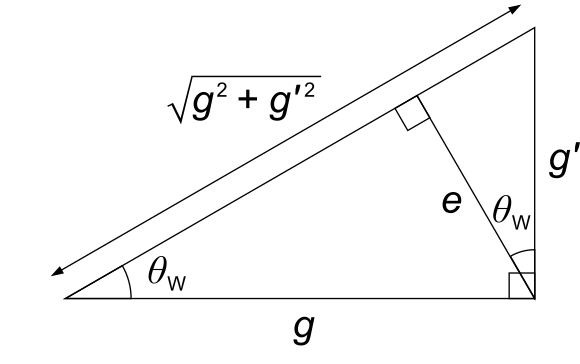
\includegraphics[width=0.5\textwidth]{figures/Weinberg_angle.png}
	\caption{The weak mixing angle $\theta_W$ is the angle relating $g'$ to $g$.}
	\label{fig:weinberg}
\end{figure}

 \begin{figure}[h!]
\centering
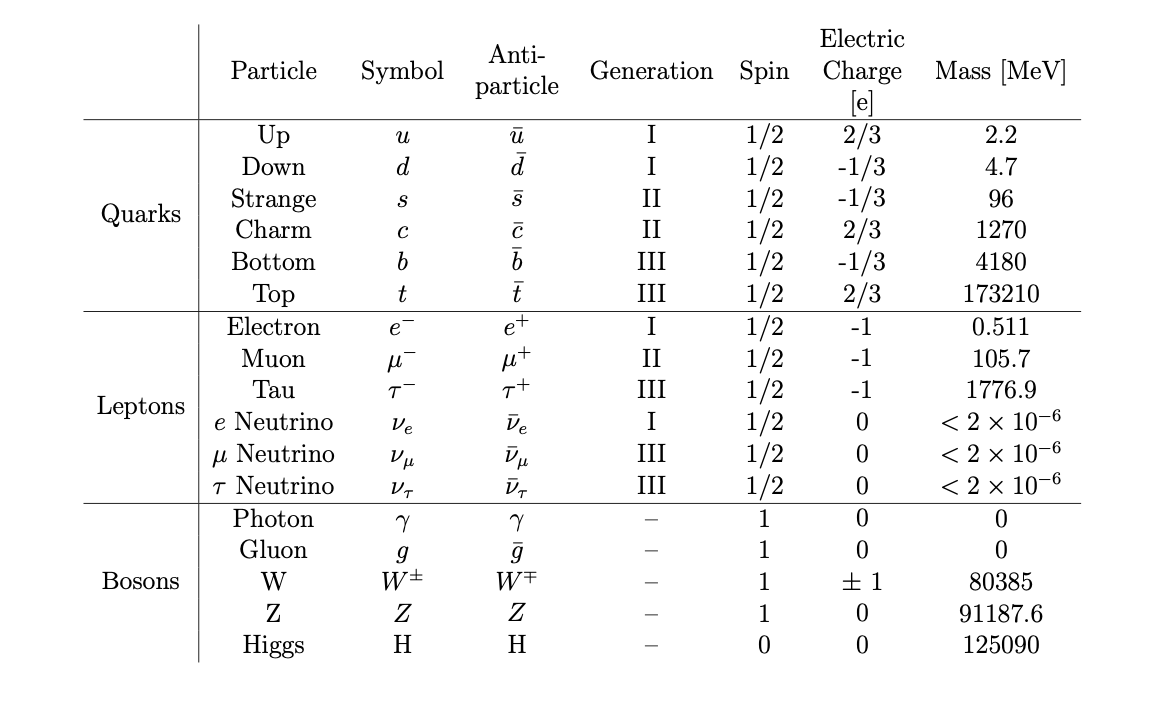
\includegraphics[width=0.8\textwidth]{figures/sm_table.png}
\caption{Table of SM particle interactions \textbf{to be replaced}.}
\label{fig:smtable}
\end{figure}





\subsection{Extra Dimensions}

One of the theories introduced to explain the hierarchy problem is the Kaluza-Klein gluon with an extra spacial dimension from the Randall-Sundrum (RS) framework. In the RS framework, there are two planes - the UV plane and the IR plane. The Planck scale is located on the UV plane, and the TeV scale is located on the IR plane. The two planes interact in the fifth spacial dimension, called the “bulk”. The Kaluza-Klein gluon has a signal comparable to SM QCD background with a luminosity of 100 fb$^{-1}$, which is comparable to the 137 fb$^{-1}$ luminosity of Run 2.

A diagram of the scale of the standard model forces to the planck scale is shown in Figure~\ref{fig:planck}. A diagram of the extra dimensions that are theorized to explain the large gap between the standard model forces and the Planck scale is shown in Figure~\ref{fig:rsbrane}.

\begin{figure}[h]
	\centering
	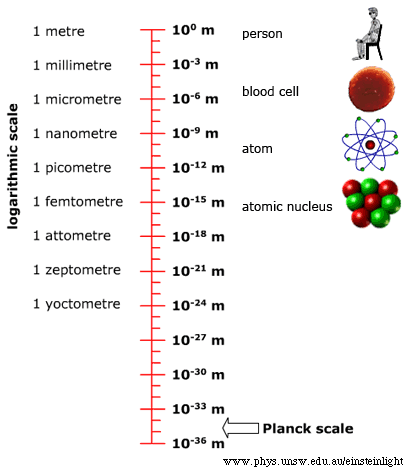
\includegraphics[width=0.5\textwidth]{figures/Planck_scale.png}
	\caption{Logarithmic scale of standard model forces and Planck scale~\cite{Planck_scale}.}
	\label{fig:planck}
\end{figure}

\begin{figure}[h]
	\centering
	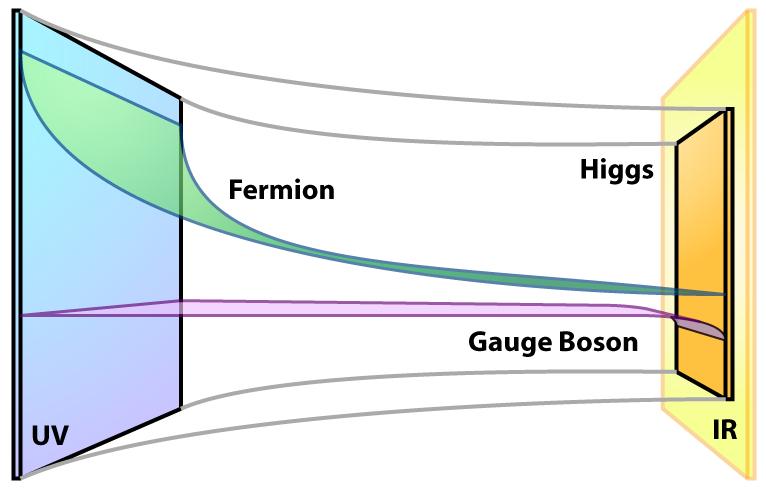
\includegraphics[width=0.75\textwidth]{figures/RSBrane.png}
	\caption{The extra spatial dimensions proposed in the Randall-Sundrum model~\cite{RSBrane}.}
	\label{fig:rsrbane}
\end{figure}

